\documentclass[aspectratio=169,11pt]{beamer}
\usepackage{beamertemplate}
\usepackage{graphicx}
\usepackage{url}
\usepackage{textcomp}
\usepackage{eurosym}
\usepackage[normalem]{ulem}
\usepackage{ragged2e}
\usepackage{etoolbox}
\apptocmd{\itemize}{\justifying}{}{}
\AtBeginEnvironment{frame}{\justifying}

% Las secciones no actuales se muestran atenuadas al 30 %
\setbeamertemplate{section in toc shaded}[default][30]

% Repite el índice al empezar cada sección, resaltando la que comienza
\AtBeginSection[]{%
  \begin{frame}{Índice}
  \small
  \tableofcontents[currentsection]
  \end{frame}
}

\title[SSI -- Tema 1.3]{Montaje de un Laboratorio de Ciberseguridad}
\subtitle{Seguridad en Sistemas Informáticos --- Tema 1.3}
\author{José Luis Martínez}
\institute{Universidad de Castilla-La Mancha}
\date{Curso 2026/27}

\begin{document}

\begin{frame}[plain]\titlepage\end{frame}

\begin{frame}{Índice}
\small
\tableofcontents
\end{frame}

\section{Introducción}

\begin{frame}[allowframebreaks]{Introducción}
\small
  \begin{itemize}
  \item Para comenzar en ciberseguridad, el primer paso es familiarizarse con herramientas, scripts o aplicaciones realizadas por terceros para realizar los primeros ejercicios
  \item PROBLEMA: Existen muchas técnicas de ataque, de reconocimiento, de post explotación y para cada una de ellas, existen multitud de herramientas que las implementas
  \item A veces, la puesta a punto de estas herramientas puede ser tediosa
  \item Cada una puedes estar implementada en diferentes lenguajes
  \item Necesidad de librerías específicas
  \item Mantenimiento y actualizaciones
  \end{itemize}
\end{frame}

\begin{frame}[allowframebreaks]{Introducción}
\small
  \begin{itemize}
  \item Existen distribuciones, basadas en Linux, que incorporar una suite completa de herramientas de seguridad, perfectamente funcionales y con ``fácil'' actualización
  \item Ejemplos:
  \item Kali Linux (\href{https://www.kali.org/}{https://www.kali.org/})
  \item Parrot SO (\href{https://www.parrotsec.org/}{https://www.parrotsec.org/})
  \item Caine (\href{https://www.caine-live.net/}{https://www.caine-live.net/})
  \item Wifislax (\href{https://www.wifislax.com/}{https://www.wifislax.com/})
  \end{itemize}
\end{frame}

\begin{frame}[allowframebreaks]{Introducción}
\small
Para desplegar las distribuciones, dos alternativas:
  \begin{itemize}
  \item Nativo en el computador
    \begin{itemize}
    \item Instalación como sistema operativo del host anfitrión
    \item Ventajas:
    \item más rápido y estable
    \item Desventaja:
    \item Usuarios poco familiarizados con Unix, puedes ser incómodo
    \end{itemize}
  \item Virtualizado
    \begin{itemize}
    \item Corren en tu sistema operativo anfitrión (un Windows, por ejemplo) de manera virtual sobre un hypervisor
    \item Ventajas:
    \item Mantiene tu PC con su configuración natural
    \item Desventaja:
    \item Más inestable, se necesitan más recursos,\dots{}
    \end{itemize}
  \end{itemize}
\end{frame}



\begin{frame}[allowframebreaks]{Introducción}
\small
Hypervisores:
  \begin{itemize}
  \item VirtualBox (\href{https://www.virtualbox.org/}{https://www.virtualbox.org/})
    \begin{itemize}
    \item VMWare (\href{https://www.vmware.com/es.html}{https://www.vmware.com/es.html})
    \end{itemize}
  \item Mi recomendación:
    \begin{itemize}
    \item para usuarios nóveles, usar un hipervisor
    \item para usuarios con destreza en sistemas unix, podéis animaros a probarlo como SSOO anfitrión
    \end{itemize}
  \end{itemize}
\end{frame}

\section{Modo hypervisor}

\begin{frame}{Modo hypervisor}
\small
Importar servicio virtualizado (carga .ova). Configuración recomendada:
\begin{columns}[t]
\begin{column}{0.48\textwidth}
\begin{center}
Habilitar PAE/NX\\[0.5ex]

\includegraphics[width=\textwidth,height=0.62\textheight,keepaspectratio]{img/sl008.png}
\end{center}
\end{column}
\begin{column}{0.48\textwidth}
\begin{center}
Deshabilitar el audio\\[0.5ex]

\includegraphics[width=\textwidth,height=0.62\textheight,keepaspectratio]{img/sl009.png}
\end{center}
\end{column}
\end{columns}
\end{frame}

\begin{frame}{Modo hypervisor}
\small
\begin{columns}[c]
\begin{column}{0.42\textwidth}
  \begin{itemize}
  \item Importar servicio virtualizado (carga .ova)
  \item Configuración: Adaptador de red
    \begin{itemize}
    \item modo puente: tenemos una IP del mismo segmento de red que la máquina anfitrión (donde corre virtualbox)
    \end{itemize}
  \end{itemize}
\end{column}
\begin{column}{0.56\textwidth}
\begin{center}
\includegraphics[width=\textwidth,height=0.8\textheight,keepaspectratio]{img/sl010.png}
\end{center}
\end{column}
\end{columns}
\end{frame}

\begin{frame}{Modo hypervisor}
\small
\begin{columns}[c]
\begin{column}{0.45\textwidth}
  \begin{itemize}
  \item Importar servicio virtualizado (carga .ova)
  \item Configuración: Adaptador de red
  \item Red NAT: El host anfitrión crea una red NAT con Ips privadas en la que estará el host virtualizado. El host hace de Gateway
  \item Necesario crear la red nat en el menú VirtualBox->Preferencias->red
  \end{itemize}
\end{column}
\begin{column}{0.53\textwidth}
\begin{center}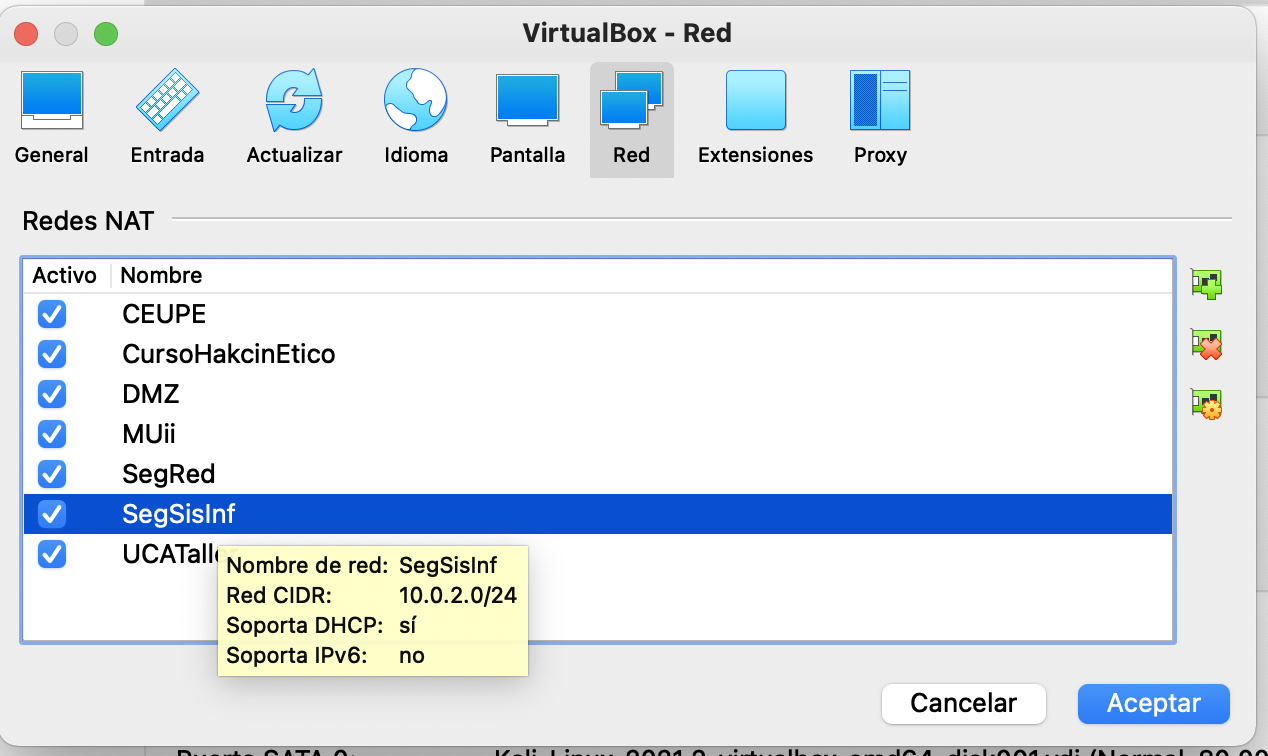
\includegraphics[width=\textwidth,height=0.8\textheight,keepaspectratio]{img/sl011.png}
\end{center}
\end{column}
\end{columns}
\end{frame}

\begin{frame}{Modo hypervisor}
\small
Arrancamos la Máquina:
\begin{columns}[c]
\begin{column}{0.42\textwidth}
  \begin{itemize}
  \item user: kali y pass: kali
  \item Actualizar:
    \begin{itemize}
    \item sudo apt-get update
    \item sudo apt-get upgrade
    \item sudo apt-get install -y virtualbox-guest-x11
    \end{itemize}
    \item Añadir además esta opción:
  \end{itemize}
\end{column}
\begin{column}{0.56\textwidth}
\begin{center}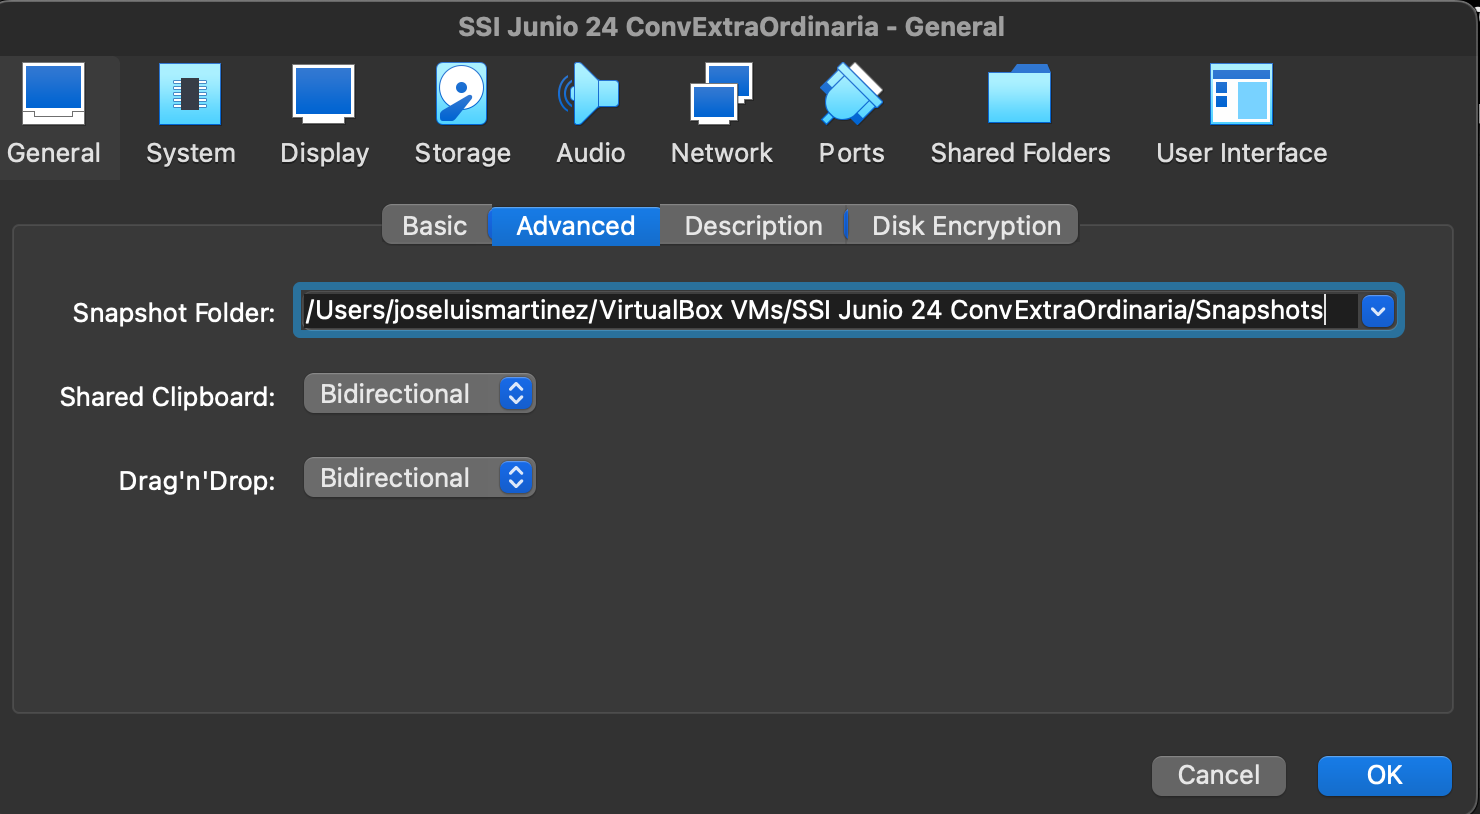
\includegraphics[width=\textwidth,height=0.8\textheight,keepaspectratio]{img/sl012.png}
\end{center}
\end{column}
\end{columns}
\end{frame}

\begin{frame}[allowframebreaks]{Modo hypervisor}
\small
Mejorar tamaño de la barra de\dots{}
  \begin{itemize}
  \item Mejorar tamaño de la barra de tareas, tamaño de letra de la terminal
  \item Cambiar el teclado de inglés a castellano
    \begin{itemize}
    \item setxkmap es
    \end{itemize}
  \item Cambiarlo de manera permanente
    \begin{itemize}
    \item En el menú de aplicaciones - > Keyboard
    \item en la pestaña Layout, seleccionar teclado ``Spanish (deadtilde)''
    \end{itemize}
  \item Tamaño de ventana:
    \begin{itemize}
    \item Menu apperence
    \end{itemize}
  \end{itemize}
\end{frame}

\begin{frame}[allowframebreaks]{Modo hypervisor}
\small
Instalar herramientas interesantes
  \begin{itemize}
  \item sudo apt-get install locate
  \item sudo apt-get install gedit

  \item Cherry Tree
    \begin{itemize}
    \item \href{https://github.com/giuspen/cherrytree}{https://github.com/giuspen/cherrytree}
    \item Preferencias en Cherry Tree: fichero configuración
    \end{itemize}
  \item Lo primero de todo comprobamos la shell en la que se esta trabajando. Recuerda que \$\$ se corresponde con el pid del proceso actual.
  \item ls -l /proc/\$\$/exe
  \item Vídeos de s4vitar para tunearte el entorno como un verdadero hacker XD:
    \begin{itemize}
    \item \href{https://www.youtube.com/watch?v=mHLwfI1nHHY}{Vídeo de s4vitar (1)}
    \item \href{https://www.youtube.com/watch?v=fshLf6u8B-w&t=5279s}{Vídeo de s4vitar (2)}
    \end{itemize}
  \item \href{https://www.youtube.com/watch?v=U1w4T03B30I}{Tutorial de Kali Linux}
  \end{itemize}
\end{frame}

\begin{frame}[allowframebreaks]{Modo hypervisor}
\small
  \begin{itemize}
  \item Descargar \href{https://sourceforge.net/projects/metasploitable/files/Metasploitable2/}{Metasploitable2}
  \item \href{https://pruebasaluuclm-my.sharepoint.com/:b:/g/personal/joseluis_martinez_uclm_es/EaGv8ii7WwNFtXhS3JpV9d0Brpj-KTzk2O_3tjyfzMKUpA?e=8had09}{Metasploitable2 en Docker}
  \item \href{https://github.com/mandiant/commando-vm}{Convertir una máquina Windows en una distribución de seguridad:}
  \end{itemize}
\end{frame}


\section{TryHackMe}

\begin{frame}[allowframebreaks]{TryHackMe}
\small
  \begin{itemize}
  \item \href{https://tryhackme.com/dashboard}{TryHackMe}
  \item Registrarse con mail + password
  \item Una vez loggeado:
    \begin{itemize}
    \item Acceso
    \item Descarga fichero ovpn y ejecutarlo desde la consola:
      \begin{itemize}
      \item openvpn nombrefichero.ovpn
      \end{itemize}
    \end{itemize}
  \end{itemize}
\begin{center}
\includegraphics[width=0.72\textwidth,height=0.58\textheight,keepaspectratio]{img/sl026.png}
\end{center}
\end{frame}

\section{HackTheBox}

\begin{frame}{HackTheBox}
\small
\begin{columns}[c]
\begin{column}{0.40\textwidth}
  \begin{itemize}
  \item \href{https://www.hackthebox.com/}{HackTheBox}
  \item \href{https://academy.hackthebox.com/dashboard}{Laboratorio (máquinas):}
  \item \href{https://academy.hackthebox.com/dashboard}{Academia:}
  \item Pasos:
    \begin{itemize}
    \item Descargar fichero ovpn
    \item Establecer la conexión con HTB con:
    \item openvpn fichero.ovpn
    \end{itemize}
  \end{itemize}
\end{column}
\begin{column}{0.58\textwidth}
\begin{center}
\includegraphics[width=\textwidth,height=0.8\textheight,keepaspectratio]{img/sl028.png}
\end{center}
\end{column}
\end{columns}
\end{frame}

\section{Docker}

\begin{frame}[allowframebreaks]{Docker}
\small
  \begin{itemize}
  \item Docker es una plataforma de contenedores de software que permite crear, distribuir y ejecutar aplicaciones en entornos aislados. Esto significa que se pueden empaquetar las aplicaciones con todas sus dependencias y configuraciones en un contenedor que se puede mover fácilmente de una máquina a otra, independientemente de la configuración del sistema operativo o del hardware.
  \item Algunas de las ventajas que se presentan a la hora de practicar hacking usando Docker son:
  \begin{itemize}

  \item Aislamiento: los contenedores de Docker están aislados entre sí, lo que significa que si una aplicación dentro de un contenedor es comprometida, el resto del sistema no se verá afectado.
  \item Portabilidad: los contenedores de Docker se pueden mover fácilmente de un sistema a otro, lo que los hace ideales para desplegar entornos vulnerables para prácticas de hacking.
  \item Reproducibilidad: los contenedores de Docker se pueden configurar de forma precisa y reproducible, lo que es importante en el hacking para poder recrear escenarios de ataque.
  \end{itemize}

  \end{itemize}
\end{frame}

\begin{frame}[allowframebreaks]{Docker}
\small

  A continuación, se mostrará cómo instalar Docker, cómo crear y administrar contenedores, y cómo usar Docker para desplegar entornos vulnerables para practicar hacking.


  \begin{itemize}
  \item Para instalar Docker en Linux, se puede utilizar el comando:
  \begin{itemize}
  \item apt install docker.io
  \end{itemize}
  \item Una vez que Docker ha sido instalado, es necesario iniciar el demonio de Docker para que los contenedores puedan ser creados y administrados:
  \begin{itemize}
  \item service docker start
  \end{itemize}
  
  \item Ver imágenes descargadas
  \begin{itemize}
  \item docker images
  \end{itemize}
  
  \item Descargar imágenes
  \begin{itemize}
  \item docker pull ubuntu:latest
  \end{itemize}
  
  \end{itemize}
\end{frame}

\begin{frame}[allowframebreaks]{Docker}
\small
  \begin{itemize}
  \item  Ejecutar un contenerdor
  \begin{itemize}
  \item docker run [opciones] nombre\_de\_la\_imagen
  \item ``-d'' o ``--detach``: se utiliza para arrancar el contenedor en segundo plano, en lugar de en primer plano.
  \item ``-i'' o ``--interactive``: se utiliza para permitir la entrada interactiva al contenedor.
  \item ``-t'' o ``--tty``: se utiliza para asignar un seudoterminal al contenedor.
  \item ``--name``: se utiliza para asignar un nombre al contenedor.
  \item docker run -dit mi\_imagen
  \end{itemize}
  \item Una vez que el contenedor está en ejecución, se puede utilizar el comando para listar los contenedores que están en ejecución en el sistema
    \begin{itemize}
  \item docker ps. Algunas de las opciones más comunes son:
  \item -a: se utiliza para listar todos los contenedores, incluyendo los contenedores detenidos.
  \item -q: se utiliza para mostrar sólo los identificadores numéricos de los contenedores.
   \end{itemize}

 
  \end{itemize}
\end{frame}

\begin{frame}[allowframebreaks]{Docker}
\small
  \begin{itemize}
  \item Detener un contendedor:
  \begin{itemize}
  \item docker stop identificador
  \end{itemize}
  \item Para ejecutar comandos en un contenedor que ya está en ejecución, se utiliza el comando:
  \begin{itemize}
  \item docker exec
  \item -i: se utiliza para permitir la entrada interactiva al contenedor.
  \item -t: se utiliza para asignar un seudoterminal al contenedor.
  \end{itemize}
  \item Por ejemplo, si se desea ejecutar el comando ``bash'' en el contenedor con el identificador ``123456789``, se puede utilizar la siguiente sintaxis:
  \begin{itemize}

  \item docker exec -it 123456789 bash
  \item docker exec -it 123456789 whoami
    \end{itemize}
  \end{itemize}
\end{frame}

\begin{frame}[allowframebreaks]{Docker}
\small
  \begin{itemize}
  \item En la máquina anfitrión se levanta la interfaz de red docker0 conectada a una red tipo 172.17.0.1:
    \begin{itemize}
    \item ifconfig
    \end{itemize}
  \item Problema: los contenedores vienen casi sin herramientas para proceder a instalarlas:
    \begin{itemize}
    \item apt update
    \item apt install net-tools
    \item apt install iputils-ping
    \end{itemize}
    \item docker rm \$(docker ps -a -q) --force: este comando se utiliza para eliminar todos los contenedores en el sistema, incluyendo los contenedores detenidos.
  \end{itemize}
\end{frame}

\begin{frame}[allowframebreaks]{Docker}
\small
  \begin{itemize}
  \item docker rm id\_contenedor: este comando se utiliza para eliminar un contenedor específico a partir de su identificador. Es importante tener en cuenta que la eliminación de un contenedor eliminará también cualquier cambio que se haya realizado dentro del contenedor, como la instalación de paquetes o la modificación de archivos.
  \item docker rmi \$(docker images -q): este comando se utiliza para eliminar todas las imágenes de Docker en el sistema.
  \item docker rmi id\_imagen: este comando se utiliza para eliminar una imagen específica a partir de su identificador. Es importante tener en cuenta que la eliminación de una imagen eliminará también cualquier contenedor que se haya creado a partir de esa imagen. Si se desea eliminar una imagen que tiene contenedores en ejecución, se deben detener primero los contenedores y luego eliminar la imagen.
  \end{itemize}
\end{frame}

\begin{frame}[allowframebreaks]{Docker}
\small
  \begin{itemize}
  \item El port forwarding, también conocido como reenvío de puertos, nos permite redirigir el tráfico de red desde un puerto específico en el host a un puerto específico en el contenedor. Esto nos permitirá acceder a los servicios que se ejecutan dentro del contenedor desde el exterior
  \item Docker port nombre\_imagen
  \item para ver puertos
  \item lsof --i:80
  \item Docker run -dit -p 80:80 -name mycontenedor mycontenedor
  \item Las monturas permite que un directorio local esté montado en el contendoer
    \begin{itemize}
    \item Docker run -dit -p 80:80 --v /home/pplu/descargas:/var/www/html/ --name mycontenedor mycontenderor
    \item docker run -v /home/usuario/datos:/datos mi\_imagen
    \end{itemize}
  \end{itemize}
\end{frame}


\begin{frame}[allowframebreaks]{Docker}
\small
Dockerfile
  \begin{itemize}
  \item Es un archivo Dockerfile se compone de varias secciones, cada una de las cuales comienza con una palabra clave en mayúsculas, seguida de uno o más argumentos.
  \item Algunas de las secciones más comunes en un archivo Dockerfile son:
  \begin{itemize}
  \item FROM: se utiliza para especificar la imagen base desde la cual se construirá la nueva imagen.
  \item RUN: se utiliza para ejecutar comandos en el interior del contenedor, como la instalación de paquetes o la configuración del entorno.
  \item COPY: se utiliza para copiar archivos desde el sistema host al interior del contenedor.
  \item CMD: se utiliza para especificar el comando que se ejecutará cuando se arranque el contenedor.
  \end{itemize}
  \end{itemize}
\end{frame}

\begin{frame}{Docker}
\small
\begin{columns}[c]
\begin{column}{0.50\textwidth}
  \begin{itemize}
  \item Además de estas secciones, también se pueden incluir otras instrucciones para configurar el entorno, instalar paquetes adicionales, exponer puertos de red y más.
    \begin{itemize}
    \item ENTRYPOINT: introduce un comando que se debe ejecutar al levantarse el contenedor
    \item EXPOSE: publica un puerto en el contenedor
    \item ENV: para crear variables de entorno
    \end{itemize}
  \item docker build -t mi\_imagen:v1 /home/usuario/proyecto/
  \end{itemize}
\end{column}
\begin{column}{0.48\textwidth}
\begin{center}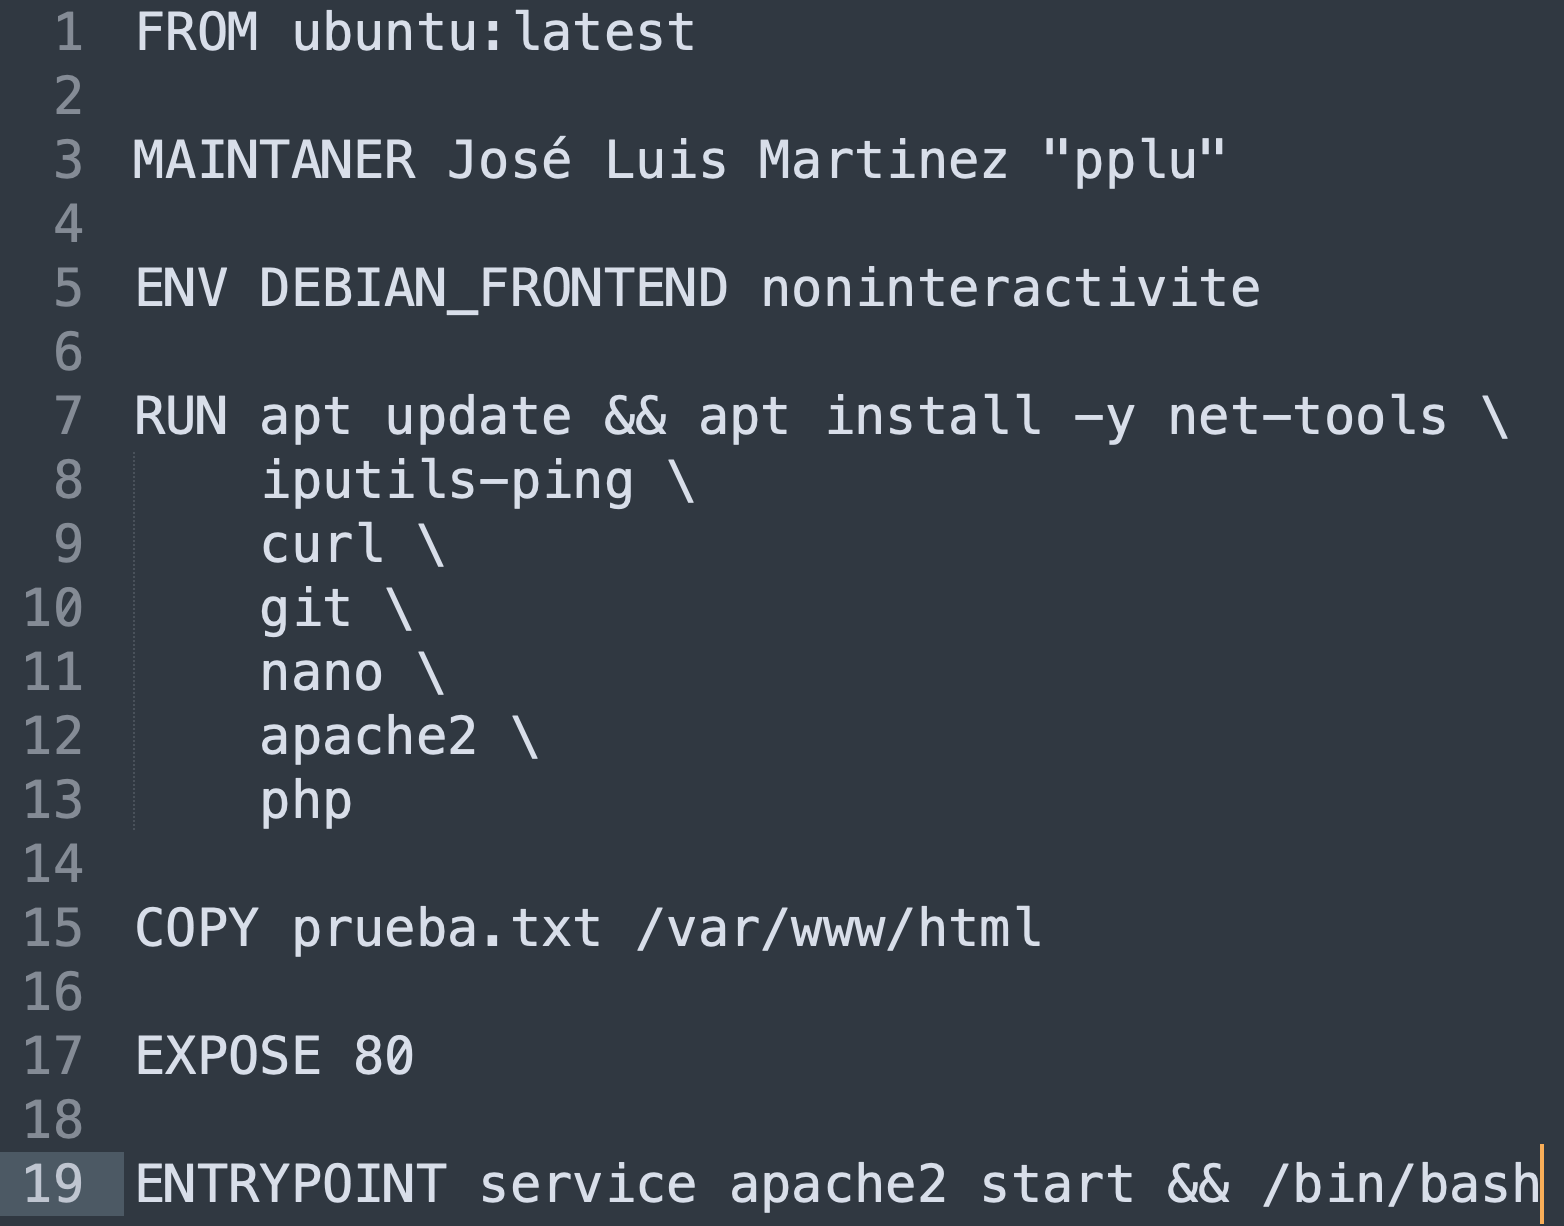
\includegraphics[width=\textwidth,height=0.8\textheight,keepaspectratio]{img/sl039.png}
\end{center}
\end{column}
\end{columns}
\end{frame}

\begin{frame}[allowframebreaks]{Ejercicio}
\small
  \begin{itemize}
  \item \href{https://tryhackme.com/room/introtodockerk8pdqk}{Resuelve este reto de TryHackMe}
  \end{itemize}
\begin{center}
\includegraphics[width=0.72\textwidth,height=0.58\textheight,keepaspectratio]{img/sl041.jpg}
\end{center}
\end{frame}

\begin{frame}[allowframebreaks]{Docker}
\small

  \begin{itemize}
  \item \href{https://www.linkedin.com/posts/deep-hacking_----el-activity-7239996426930315264-QjJO/}{Kali Linux en Docker}
  \item \href{https://www.linkedin.com/posts/ilana-aminoff_primeros-pasos-con-docker-levantar-docker-ugcPost-7358427608880930817-izYW}{Desplegar Docker en Windows}
  \item Distribuciones de seguridad basadas en Docker:
    \begin{itemize}
    \item \href{https://github.com/aaaguirrep/offensive-docker}{offensive-docker}
    \item \href{https://www.redeszone.net/2017/04/09/pwnbox-docker-herramientas-hacking/}{pwnbox}
    \item \href{https://github.com/yeswehack/pwn-machine}{pwnMachine}
    \end{itemize}
  \end{itemize}
\end{frame}

\begin{frame}[allowframebreaks]{Docker}
\small
  \begin{itemize}
  \item Docker Compose es una herramienta de orquestación de contenedores que permite definir y ejecutar aplicaciones multi-contenedor de manera fácil y eficiente. Con Docker Compose, podemos describir los diferentes servicios que componen nuestra aplicación en un archivo YAML y, a continuación, utilizar un solo comando para ejecutar y gestionar todos estos servicios de manera coordinada.
  \item En otras palabras, Docker Compose nos permite definir y configurar múltiples contenedores en un solo archivo YAML, lo que simplifica la gestión y la coordinación de múltiples contenedores en una sola aplicación. Esto es especialmente útil para aplicaciones complejas que requieren la interacción de varios servicios diferentes, ya que Docker Compose permite definir y configurar fácilmente la conexión y la comunicación entre estos servicios.
  \end{itemize}
\end{frame}

\begin{frame}[allowframebreaks]{Docker}
\small
  \begin{itemize}
  \item Repositorio:
  \item \href{https://github.com/vulhub/vulhub}{Vulhub}
  \item Cloando:
    \begin{itemize}
    \item \href{https://github.com/vulhub/vulhub/tree/master/imagemagick}{https://github.com/vulhub/vulhub/tree/master/imagemagick}
    \item svn checkout \href{https://github.com/vulhub/vulhub/trunk/imagemagick}{https://github.com/vulhub/vulhub/trunk/imagemagick}
    \end{itemize}
  \item cd ``directory''
  \item docker-compose --d up
  \end{itemize}
\end{frame}

\begin{frame}[allowframebreaks]{Docker}
\small
Comandos Docker (chuleta)
  \begin{itemize}
  \item Imágenes
  \item docker pull img $\cdot$ docker images $\cdot$ docker build -t nombre . $\cdot$ docker rmi img
  \item Contenedores
  \item docker run -d -p 8080:80 --name web img $\cdot$ docker ps -a
  \item docker exec -it web bash $\cdot$ docker stop/start/rm web $\cdot$ docker logs web
  \item Volúmenes y redes
  \item docker volume create datos (-v datos:/ruta) $\cdot$ docker network create red
  \item Docker Compose
  \item docker compose up -d $\cdot$ docker compose down $\cdot$ docker compose logs -f
  \item Flujo: build $\rightarrow$ run $\rightarrow$ exec/logs $\rightarrow$ stop/rm. Compose orquesta varios contenedores.
  \end{itemize}
\end{frame}


\section{Aplicaciones web vulnerables con Docker}

\begin{frame}[allowframebreaks]{Aplicaciones Web Vulnerables con Docker}
\small
  \begin{itemize}
  \item Entornos de práctica listos en minutos
  \item Aplicaciones clásicas
  \item DVWA --- PHP/MySQL, 10 categorías OWASP
  \item OWASP Juice Shop --- Node.js, 100+ retos
  \item OWASP WebGoat --- Java EE, lecciones guiadas
  \item SQLi-Labs --- 75 laboratorios de inyección SQL
  \item bWAPP --- PHP, +100 bugs web
  \item Mutillidae II --- LAMP, OWASP Top 10
  \item APIs y tecnologías modernas
  \item DVGA --- GraphQL, introspección, DoS
  \item DVRestaurant API --- REST, IDOR, JWT bypass
  \item PyGoat --- Django (Python), SSTI, A10
  \item Vulnerabilidades específicas
  \item SSRF Lab --- request forgery, LFI, XXE
  \item VulnBank --- IDOR, transfer forgery
  \item VulnLab --- XSS, SQL, SSRF, path traversal
  \item WrongSecrets --- secretos en config/código
  \item Zero Health API --- BOLA, mass assignment
  \item Ventajas del enfoque Docker
  \item $\rightarrow$ docker pull / docker run en segundos
  \item $\rightarrow$ Aislamiento total del host
  \item $\rightarrow$ Reset instantáneo: docker rm + docker run
  \item $\rightarrow$ Red interna entre contenedores
  \end{itemize}
\end{frame}

\begin{frame}{Aplicaciones Web Vulnerables con Docker}
\footnotesize
\begin{columns}[c]
\begin{column}{0.66\textwidth}
  \begin{itemize}
  \item DVWA --- Damn Vulnerable Web Application
  \item ¿Qué es?
  \item Aplicación PHP con MySQL diseñada para ser vulnerable
  \item 10 categorías del OWASP Top 10 en niveles: Low/Med/High/Impossible
  \item Instalación
  \item $\rightarrow$ docker pull vulnerables/web-dvwa
  \item $\rightarrow$ docker run -d -p 80:80 --name dvwa \textbackslash{}
  \item vulnerables/web-dvwa
  \item Primer acceso
  \item $\rightarrow$ http://localhost/setup.php $\rightarrow$ Create/Reset Database
  \item Login por defecto: admin / password
  \end{itemize}
\end{column}
\begin{column}{0.32\textwidth}
\begin{center}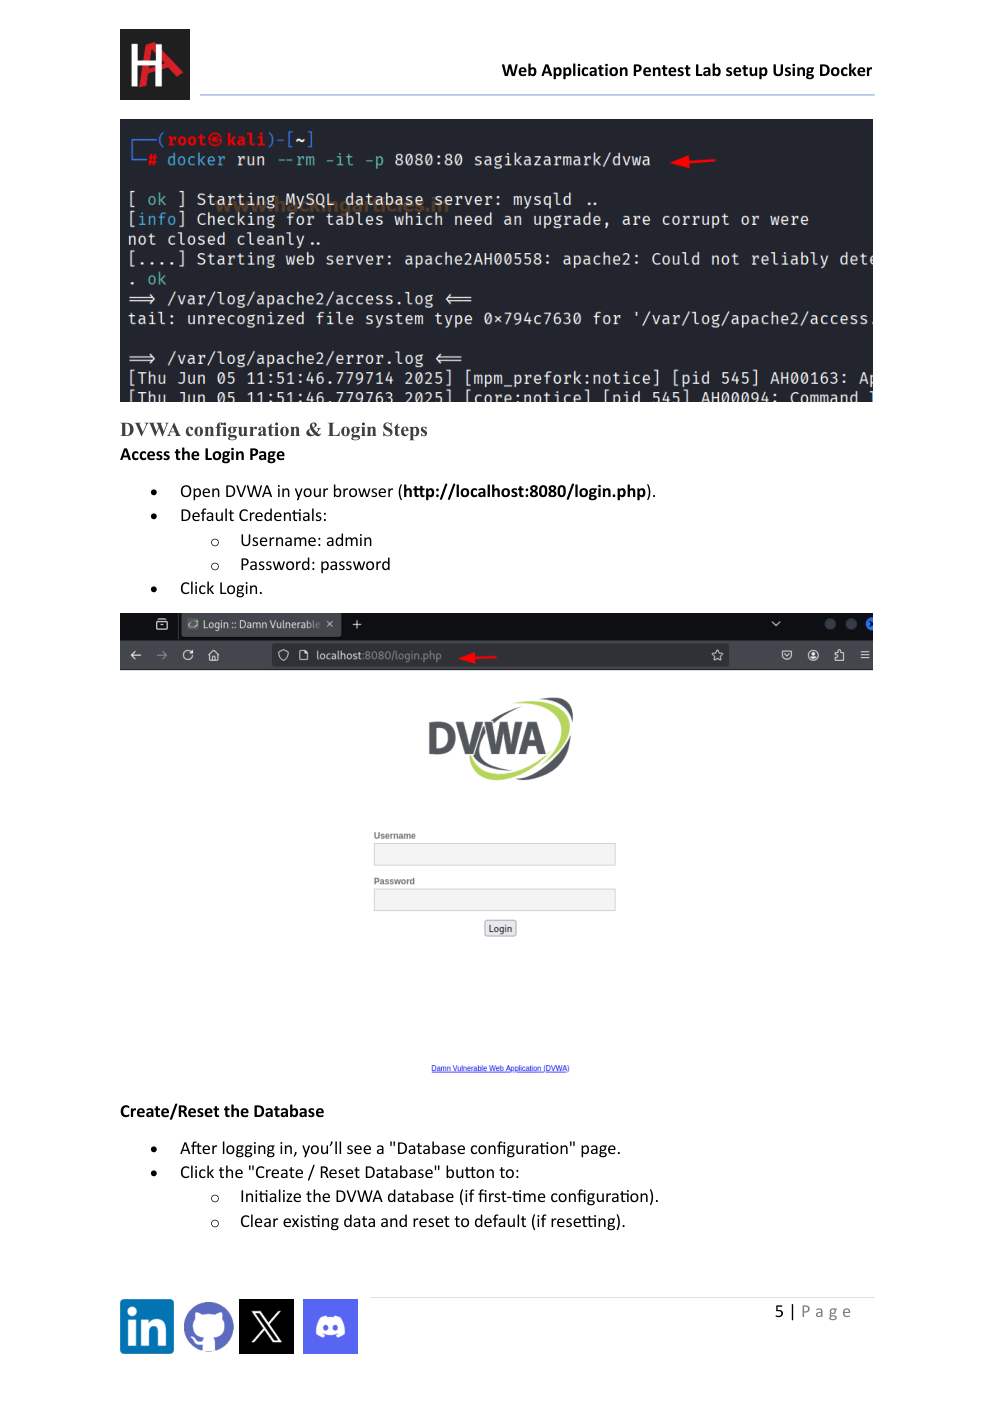
\includegraphics[width=\textwidth,height=0.85\textheight,keepaspectratio]{img/sl050.png}
\end{center}
\end{column}
\end{columns}
\end{frame}

\begin{frame}{Aplicaciones Web Vulnerables con Docker}
\footnotesize
\begin{columns}[c]
\begin{column}{0.66\textwidth}
  \begin{itemize}
  \item OWASP Juice Shop
  \item CTF-style con más de 100+ retos
  \item Score board oculto --- parte del reto es encontrarlo
  \item Instalación
    \begin{itemize}
    \item $\rightarrow$ docker pull bkimminich/juice-shop
    \item $\rightarrow$ docker run -d -p 3000:3000 --name juiceshop \textbackslash{}bkimminich/juice-shop
    \end{itemize}
  \item Primer acceso $\rightarrow$ http://localhost:3000
  \item Categorías
  \item XSS, SQLi, Broken Auth, IDOR, Broken Access Control, Sensitive Data Exposure, XXE, Insecure Deserialization
  \item Retos especiales: Criptografía, JWT, OAuth2
  \end{itemize}
\end{column}
\begin{column}{0.32\textwidth}
\begin{center}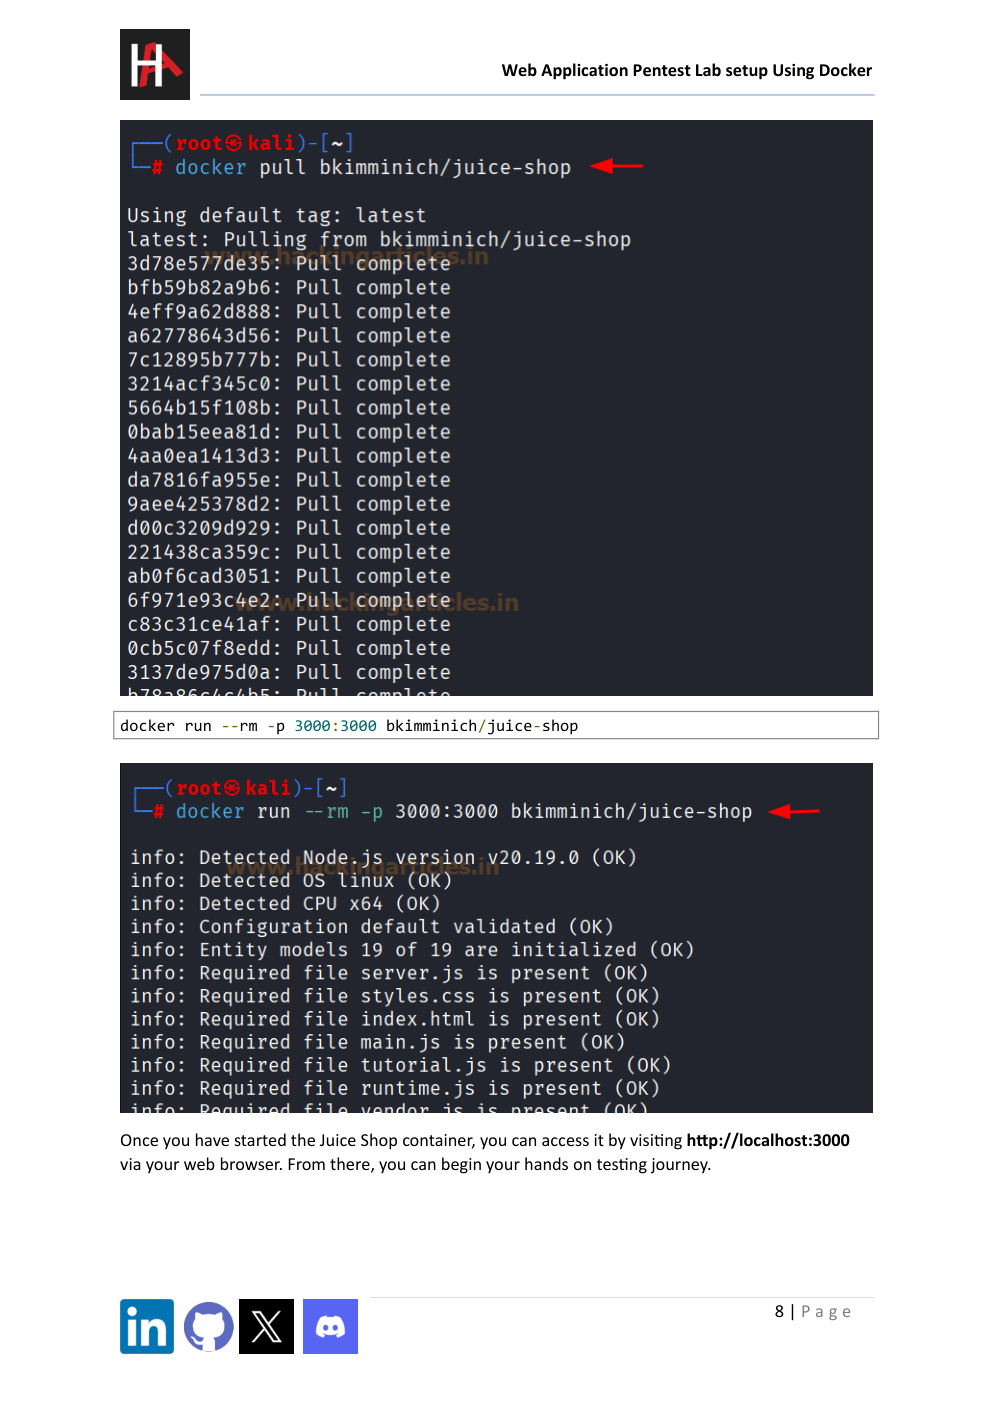
\includegraphics[width=\textwidth,height=0.85\textheight,keepaspectratio]{img/sl051.png}
\end{center}
\end{column}
\end{columns}
\end{frame}

\begin{frame}{Aplicaciones Web Vulnerables con Docker}
\footnotesize
\begin{columns}[c]
\begin{column}{0.66\textwidth}
  \begin{itemize}
  \item OWASP WebGoat
  \item Plataforma de aprendizaje con lecciones interactivas. Explica la vulnerabilidad y luego te pide explotarla
  \item Java EE $\cdot$ Spring $\cdot$ Puerto 8080
  \item Instalación
    \begin{itemize}
    \item $\rightarrow$ docker pull webgoat/goat-and-wolf
    \item $\rightarrow$ docker run -d -p 8080:8080 --name webgoat \textbackslash{} webgoat/goat-and-wolf
    \end{itemize}
  \item Primer acceso $\rightarrow$ http://localhost:8080/WebGoat
  \item Injection, Broken Auth, XSS, Insecure Direct Object Refs, Security Misconfiguration, Vulnerable Components, CSRF/SSRF, Insecure Deserialization
  \end{itemize}
\end{column}
\begin{column}{0.32\textwidth}
\begin{center}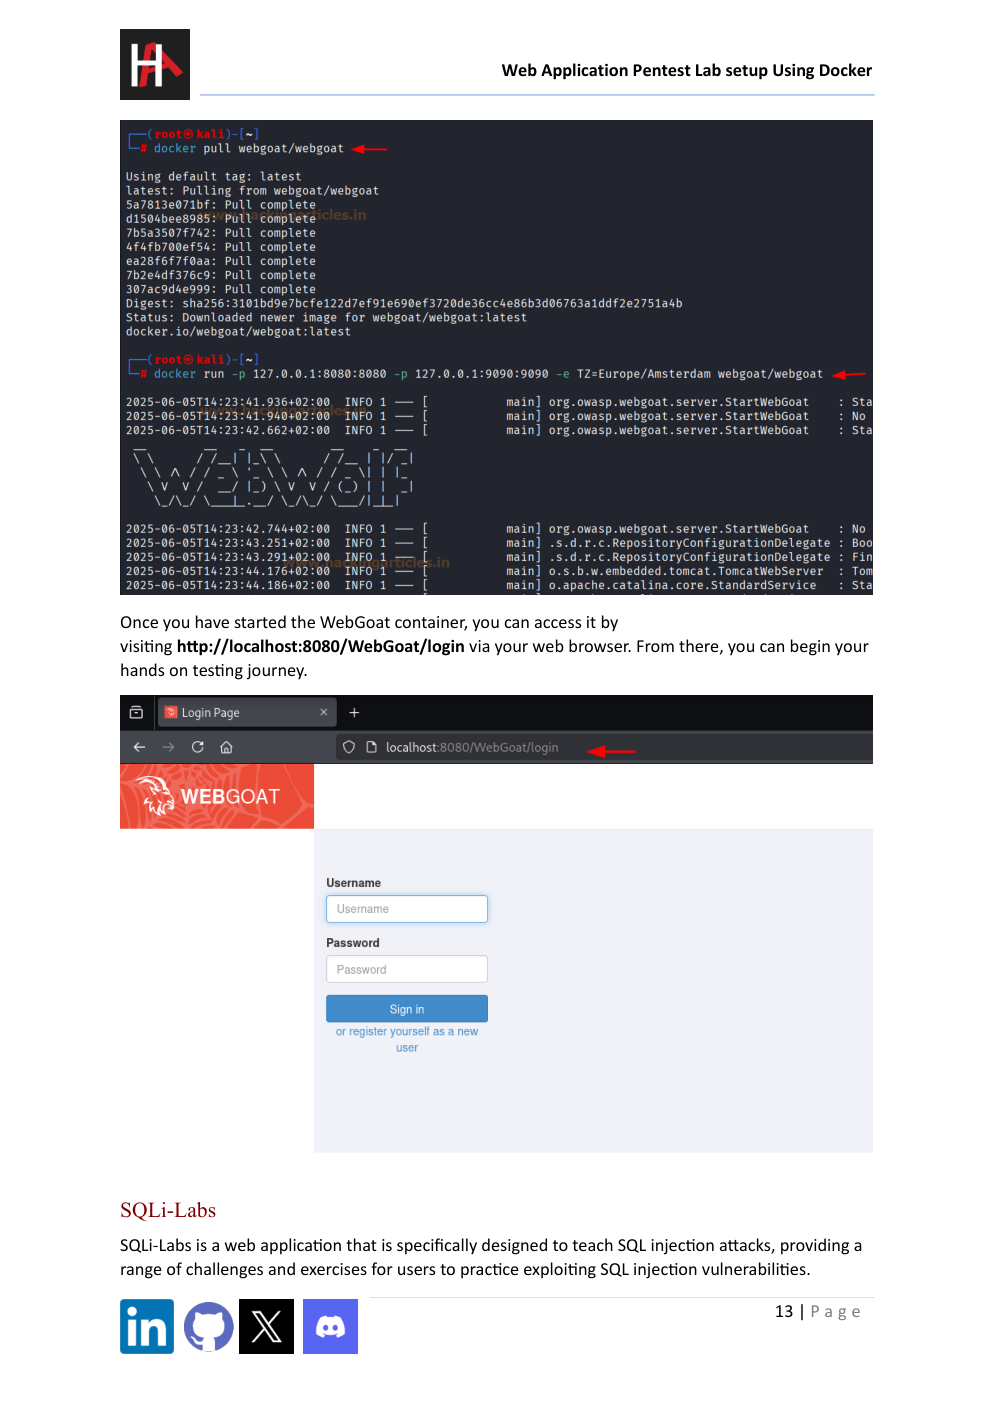
\includegraphics[width=\textwidth,height=0.85\textheight,keepaspectratio]{img/sl052.png}
\end{center}
\end{column}
\end{columns}
\end{frame}

\begin{frame}{Aplicaciones Web Vulnerables con Docker}
\footnotesize
\begin{columns}[c]
\begin{column}{0.66\textwidth}
  \begin{itemize}
  \item SQLi-Labs
  \item PHP $\cdot$ MySQL $\cdot$ 75 laboratorios
  \item SQL Injection $\cdot$ Error-based $\cdot$ Time-based
  \item Instalación
    \begin{itemize}
    \item $\rightarrow$ docker pull acgpiano/sqli-labs
    \item $\rightarrow$ docker run -d -p 80:80 --name sqli \textbackslash{} acgpiano/sqli-labs
    \end{itemize}
  \item Primer acceso $\rightarrow$ http://localhost/sql-connections/setup-db.php
  \item $\rightarrow$ http://localhost/Less-1/?id=1
  \end{itemize}
\end{column}
\begin{column}{0.32\textwidth}
\begin{center}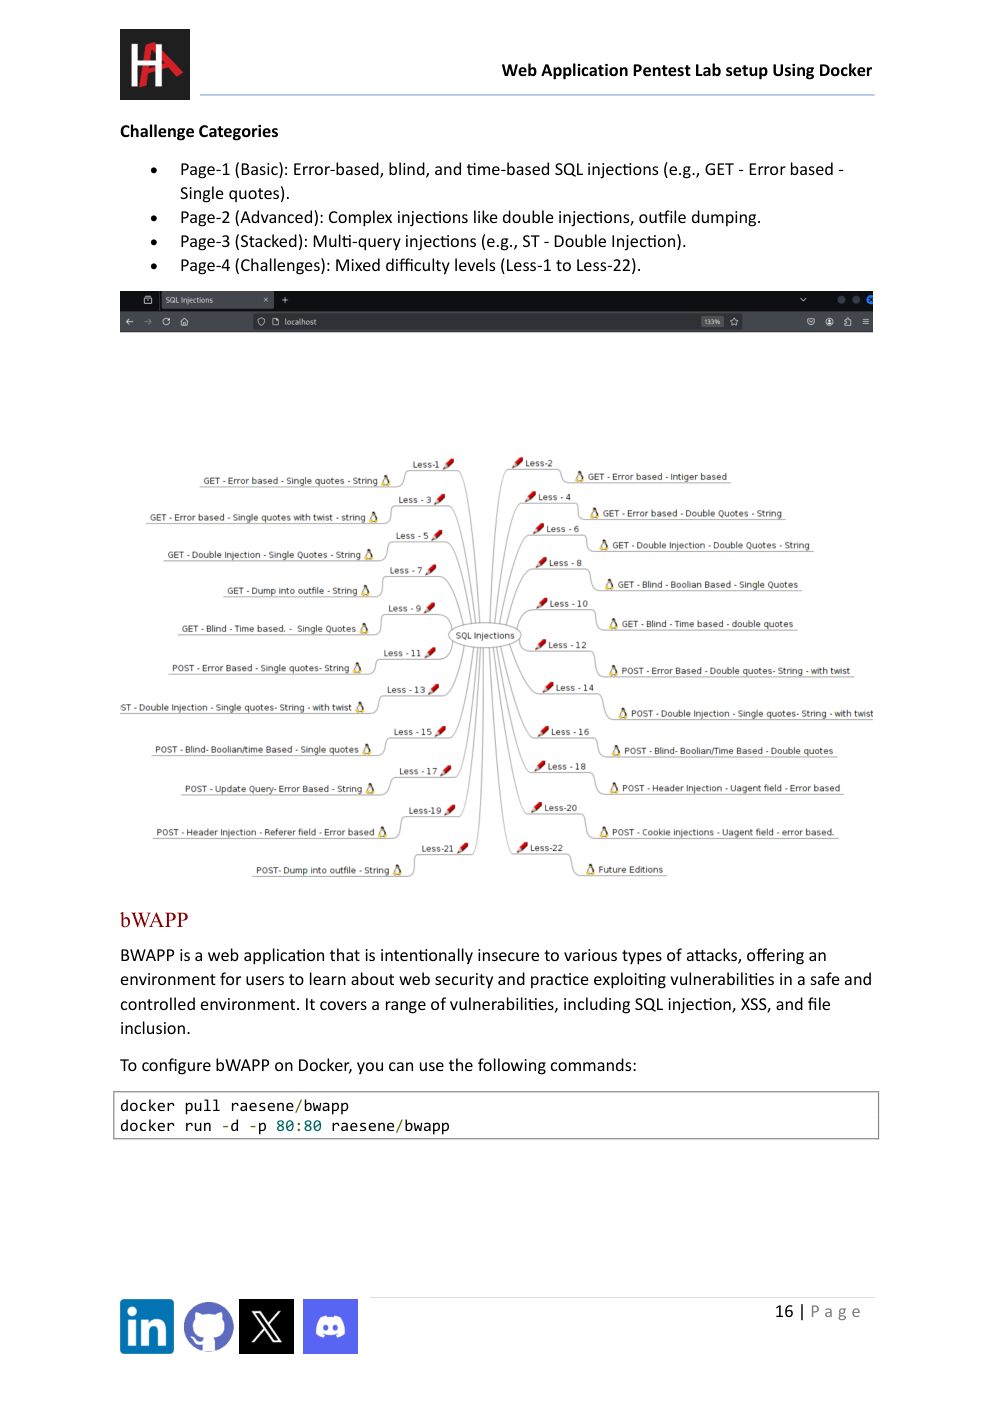
\includegraphics[width=\textwidth,height=0.85\textheight,keepaspectratio]{img/sl053.png}
\end{center}
\end{column}
\end{columns}
\end{frame}

\begin{frame}[allowframebreaks]{Aplicaciones Web Vulnerables con Docker}
\small
  \begin{itemize}
  \item bWAPP + Mutillidae II
  \item +100 vulnerabilidades web, niveles: low/medium/high
  \item Instalación:
     \begin{itemize}
  \item $\rightarrow$ docker pull raesene/bwapp
  \item $\rightarrow$ docker run -d -p 80:80 --name bwapp raesene/bwapp
  \item $\rightarrow$ http://localhost/install.php $\rightarrow$ Click here to install bWAPP
    \end{itemize}
  \item Login: bee / bug
  \item Mutillidae II
  \item Instalación:
  \begin{itemize}
  \item $\rightarrow$ docker pull webpwnized/mutillidae
  \item $\rightarrow$ docker run -d -p 80:80 --name mutillidae \textbackslash{}
  \item webpwnized/mutillidae
  \item $\rightarrow$ http://localhost/mutillidae
  \end{itemize}
  \end{itemize}
\begin{center}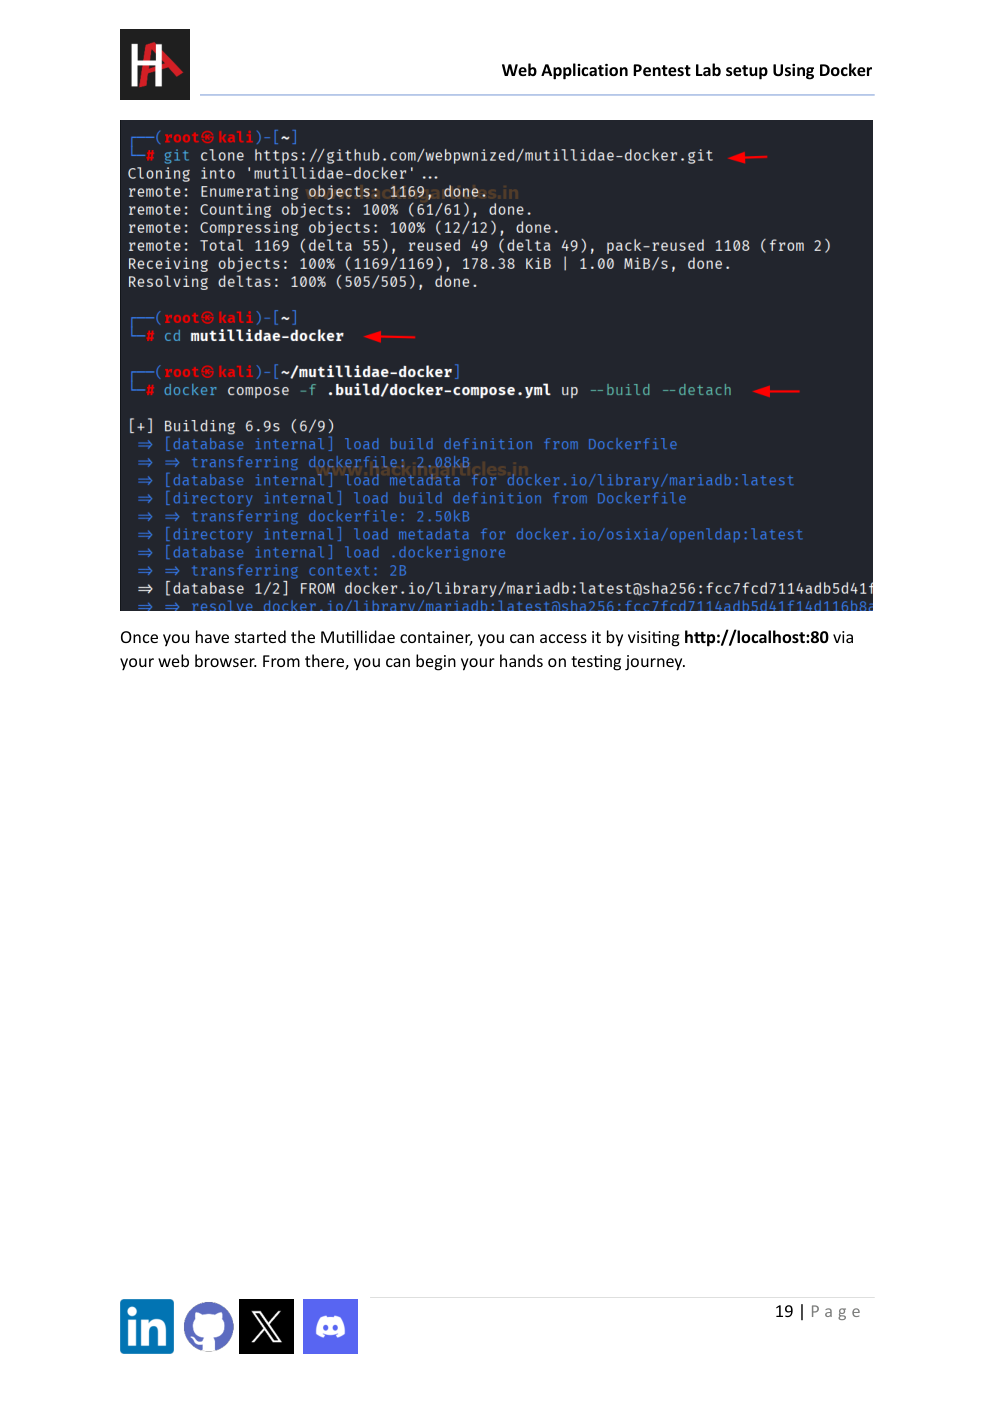
\includegraphics[width=0.72\textwidth,height=0.58\textheight,keepaspectratio]{img/sl054.png}
\end{center}
\end{frame}

\begin{frame}{Aplicaciones Web Vulnerables con Docker}
\footnotesize
\begin{columns}[c]
\begin{column}{0.66\textwidth}
  \begin{itemize}
  \item APIs Vulnerables: DVGA + DVRestaurant
  \item GraphQL $\cdot$ REST API $\cdot$ JWT $\cdot$ IDOR
  \item Instalación DVGA:
    \begin{itemize}
    \item $\rightarrow$ docker pull dolevf/dvga
    \item $\rightarrow$ docker run -d -p 5013:5013 --name dvga dolevf/dvga
    \item $\rightarrow$ http://localhost:5013
    \end{itemize}
  \item Modo fácil: header X-DVGA-MODE: Beginner
  \item Instalación DVRestaurant API
    \begin{itemize}
    \item $\rightarrow$ docker pull thomasdotbiz/dvrestaurant
    \item $\rightarrow$ docker run -d -p 3001:3001 --name dvrest thomasdotbiz/dvrestaurant
    \item $\rightarrow$ http://localhost:3001/api/docs (Swagger UI)
    \end{itemize}
  \end{itemize}
\end{column}
\begin{column}{0.32\textwidth}
\begin{center}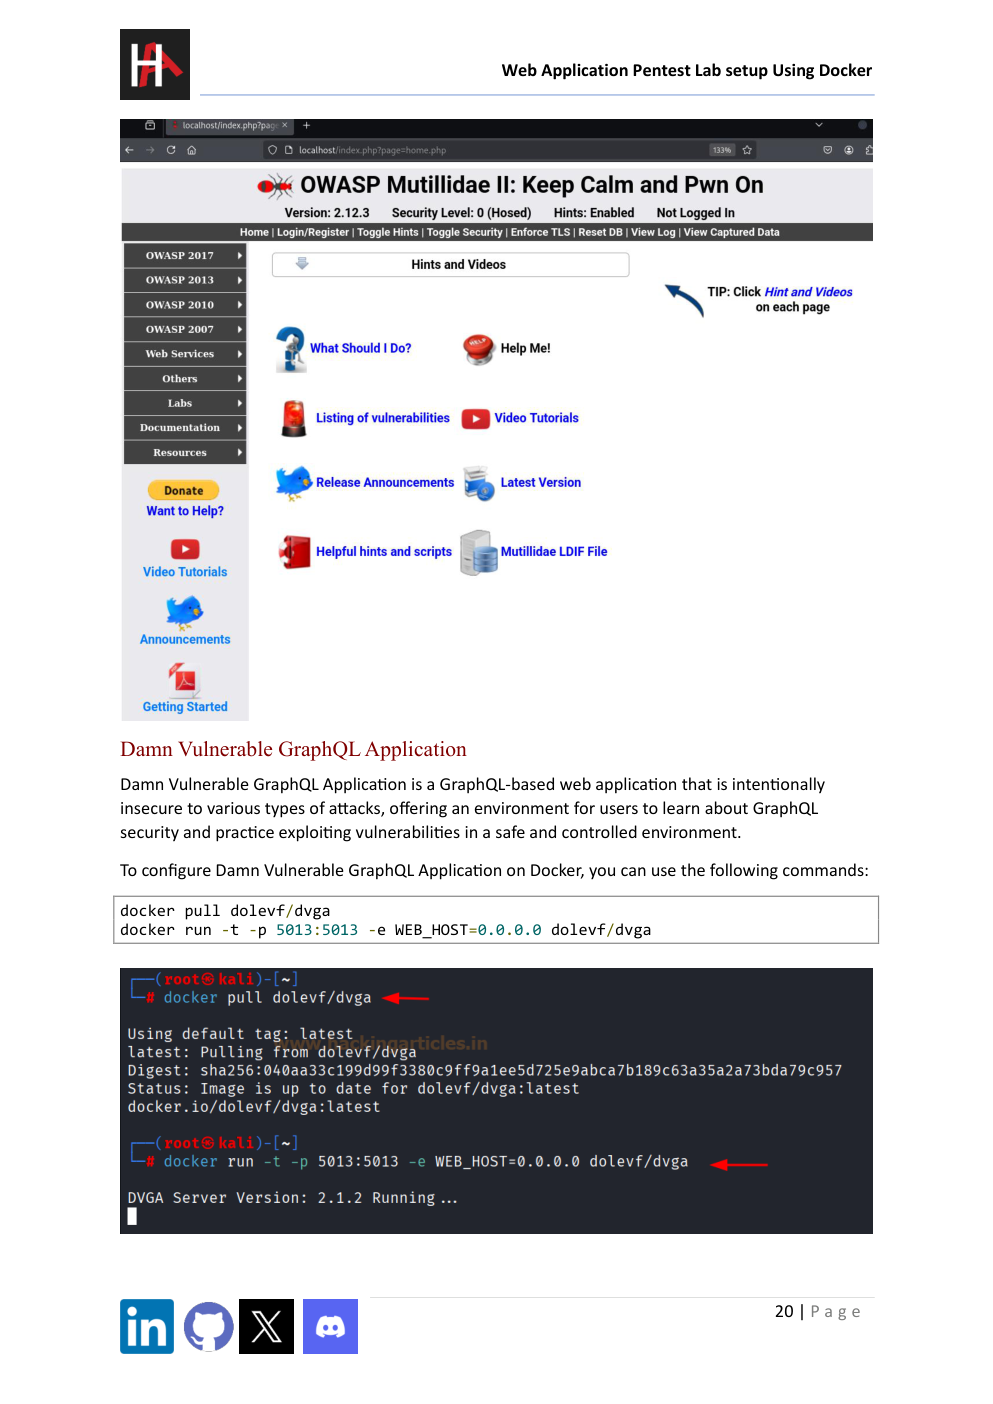
\includegraphics[width=\textwidth,height=0.85\textheight,keepaspectratio]{img/sl055.png}
\end{center}
\end{column}
\end{columns}
\end{frame}



\section{Repositorios de máquinas y retos}

\begin{frame}[allowframebreaks]{Repositorio}
\small
  \begin{itemize}
  \item Vulhub:
    \begin{itemize}
    \item \href{https://www.vulnhub.com/}{https://www.vulnhub.com}
    \end{itemize}
  \item Hackmyvm:
    \begin{itemize}
    \item \href{https://hackmyvm.eu/}{https://hackmyvm.eu}
    \end{itemize}
  \item TheHackerLab:
    \begin{itemize}
    \item \href{https://thehackerslabs.com/}{https://thehackerslabs.com}
      \begin{itemize}
      \item Máquinas: \href{https://thehackerslabs.com/seguridad-ofensiva/}{https://thehackerslabs.com/seguridad-ofensiva/}
      \item Contenedores (Docker): \href{https://dockerlabs.es/}{https://dockerlabs.es}
      \end{itemize}
    \end{itemize}
  \item PentesterLab:
    \begin{itemize}
    \item \href{https://pentesterlab.com/exercises}{https://pentesterlab.com/exercises}
    \item (algunos son free)
    \end{itemize}
  \item Offsec:
    \begin{itemize}
    \item \href{https://portal.offsec.com/dashboard}{https://portal.offsec.com/dashboard}
    \end{itemize}
  \end{itemize}
\end{frame}

\begin{frame}[plain]
  \begin{center}
    {\Huge\bfseries\color{uznavy} ¡Gracias!}\\[1em]
    {\large Seguridad en Sistemas Informáticos --- Tema 1.3}
  \end{center}
\end{frame}

\end{document}